\section{Overview}
Modeling is a powerful tool in synthetic biology and engineering. Mmodeling has provided us with an important engineering approach to characterize our pathways and predict their performance, thus helped us with modifying and testing our designing.

Basically, the models built by us can be divided into two parts.

On kinetic model parts, we hope to gain insight of the gene expression dynamics of our whole circuit. And also we tried to better characterize our parts, analyze our experimental data,and protein transport and concentration changes throughout the whole process. Several tools including ODEs and interpolation are employed.

\section{Brief introduction}
Concerned about the pollutions caused by heavy metals released by manufacturers and industries to the environment including air, water and soil and causing great harm to people’s health, we are planning to utilise an engineered microorganism to detect the existence of heavy metals, aiming to develop a novel, highly sensitive and user-friendly detection device. We will engineer and construct detection and reporter circuits into E. coli and utilise CRISPR system to modify the expression of the reporter, smURFP, a kind of fluorescent protein. The change of the level of fluorescence released from smURFP will signal the existence of heavy metals. Our goal is to improve the sensitivity of the device to a great extent to guarantee the practicability and convenience of it.
\section{Kinetic model}
\subsection{analysis of the problem}

\begin{figure}[h]
\centering
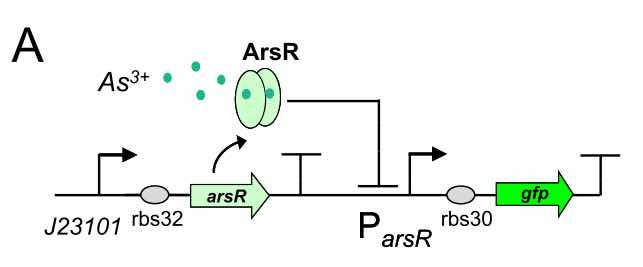
\includegraphics[width=12cm,height=5cm]{1}
\caption{Schematic diagram of plasmid1}
\end{figure}

At the beginning, on the plasmid1, the promoter $P_{arsR}$ isn't bound with ArsR, and thus active. And ArsR and $smURFP_l$ are transcribed from the promoter $P_{arsR}$. $smURFP_l$ means leaking expression without the expression of $As^{3+}$.Then ArsR will bind with the promoter $P_{arsR}$ and make it inactive. 

\begin{equation}
P_{J23104} \stackrel{k_1}{\longrightarrow} P_{J23104}+ArsR
\end{equation}

\begin{equation}
P_{arsR} \stackrel{k_2}{\longrightarrow} P_{arsR} +smURFP
\end{equation}

\begin{equation}
ArsR+P_{arsR} \xrightleftharpoons[k_{-3}]{k_3}ArsR*P_{arsR} 
\end{equation} 

On the plasmid 2, fusion protein of dcas9(dead Cas9, a mutant of Cas9) and RNAP(RNA polymerase) are produced after transcription.

\begin{equation}
P_{tet} \stackrel{k_{4}}{\longrightarrow} P_{tet} +dCas9-RNAP
\end{equation}

\begin{equation}
P_{tet} \stackrel{k_{5}}{\longrightarrow} P_{tet} +sgRNA
\end{equation}

\begin{figure}[h]
	\centering
	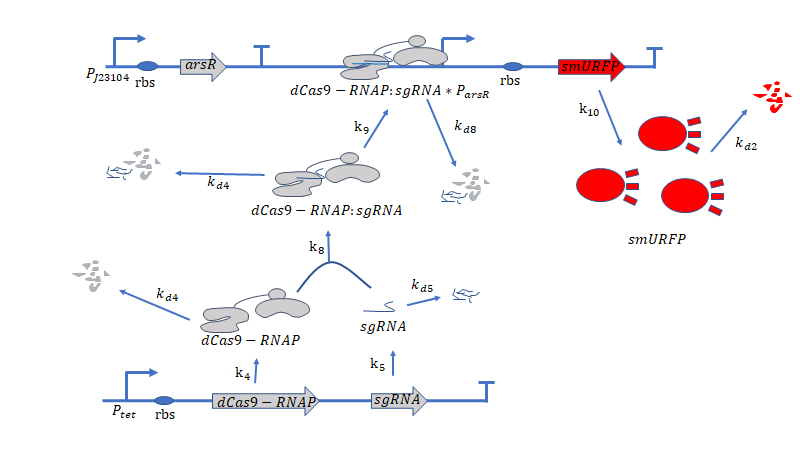
\includegraphics[width=12cm,height=5cm]{2}
	\caption{Schematic diagram of dCas9/RNAP}
\end{figure}

dCas9/RNAP can bind with it's target DNA sequence(upstream of promoter sequence) but not cut it. Simultaneously, dCas9 should have led RNAP to bind to the promoter $P_{arsR_d}$ and enhanced the transcription of GFP. However, the promoter $P_{arsR}$ has already bound with ArsR, as a result, RNAP can't bind with the promoter $P_{arsR}$ . \\ 

However, at the presence of $As^{3+}$, $As^{3+}$ can bind with ArsR, then dissociate ArsR and $P_{arsR_d}$, and combine RNAP and $P_{arsR_d}$. \\

(Declaration: $[dCas9/RNAP] = [dCas9] = [RNAP]$ ; $[P_{arsR_d}] = [P_{arsR_u}] = \frac{1}{2}[P_{arsR}]$ )

\begin{equation}
ArsR +As^{3+}\xrightleftharpoons[k_{-6}]{k_6}As^{3+}*ArsR
\end{equation}

\begin{equation}
ArsR*P_{arsR} +As^{3+}\xrightleftharpoons[k_{-7}]{k_7}P_{arsR}+ As^{3+}*ArsR
\end{equation}

\begin{equation}
dCas9-RNAP+sgRNA\xrightleftharpoons[k_{-8}]{k_8} dCas9-RNAP:sgRNA
\end{equation}

\begin{equation}
dCas9-RNAP:sgRNA+P_{arsR}\xrightleftharpoons[k_{-9}]{k_9} dCas9-RNAP:sgRNA*P_{arsR}
\end{equation}

\begin{equation}
dCas9-RNAP:sgRNA*P_{arsR}\stackrel{k_{10}}{\longrightarrow} dCas9-RNAP:sgRNA*P_{arsR}+smURFP
\end{equation}
\\\\
Take the degration into account
\\\\
\begin{equation}
ArsR\stackrel{k_{d1}}{\longrightarrow}Ø
\end{equation}

\begin{equation}
smURFP\stackrel{k_{d2}}{\longrightarrow}Ø
\end{equation}


\begin{equation}
ArsR*P_{arsR}\stackrel{k_{d3}}{\longrightarrow}P_{arsR}
\end{equation}

\begin{equation}
As^{3+}*ArsR\stackrel{k_{d4}}{\longrightarrow}As^{3+}
\end{equation}

\begin{equation}
dCas9-RNAP\stackrel{k_{d5}}{\longrightarrow}Ø
\end{equation}

\begin{equation}
sgRNA\stackrel{k_{d6}}{\longrightarrow}
\end{equation}

%\begin{equation}
%dCas9-RNAP:sgRNA\stackrel{k_{d7}}{\longrightarrow}dCas9-RNAP
%\end{equation}

\begin{equation}
dCas9-RNAP:sgRNA\stackrel{k_{d7}}{\longrightarrow}Ø
\end{equation}

%\begin{equation}
%dCas9-RNAP:sgRNA*P_{arsR}\stackrel{k_{d8}}{\longrightarrow}dCas9-RNAP+P_{arsR}
%\end{equation}

\begin{equation}
dCas9-RNAP:sgRNA*P_{arsR}\stackrel{k_{d8}}{\longrightarrow}P_{arsR}
\end{equation}
\\\\
\begin{table}[htbp]
	\centering
	\caption{\label {tab:test} Parameters}
	\begin{tabular}{cccccccccccccccccc}
		\toprule
		Rate constants & Value& units \\
		\midrule
		k1 & 1.999e-5 &1/s \\
		k2 & 3.312e-6 &1/s \\
		k3 & 3.3e7    & 1/M    \\
		k4 &1.995e-5 &1/s\\
		k5 & 3.312e-6 &1/s \\
		k6 &1.66e7   &1/M  \\
		k7  &1.26e4 &1/s  \\
		k8&1.6e-2& 1/s\\
		k9 &1.66e-5&1/s\\ 
		k10&4e-5&1/s\\
		kd1 & 3.07e-3&1/s\\
		kd2&1e-5&1/s\\
		kd3&1e-3&1/s\\
		kd4&1.53e-3&1/s\\
		kd5 & 2e-2&1/s\\
		kd6&7.62e-3&1/s\\
		kd7& 1e-2&1/s\\
		kd8&1e-1&1/s\\		
		\bottomrule
	\end{tabular}
\end{table}



\subsection{simulation }
\begin{figure}[h]
	\centering
	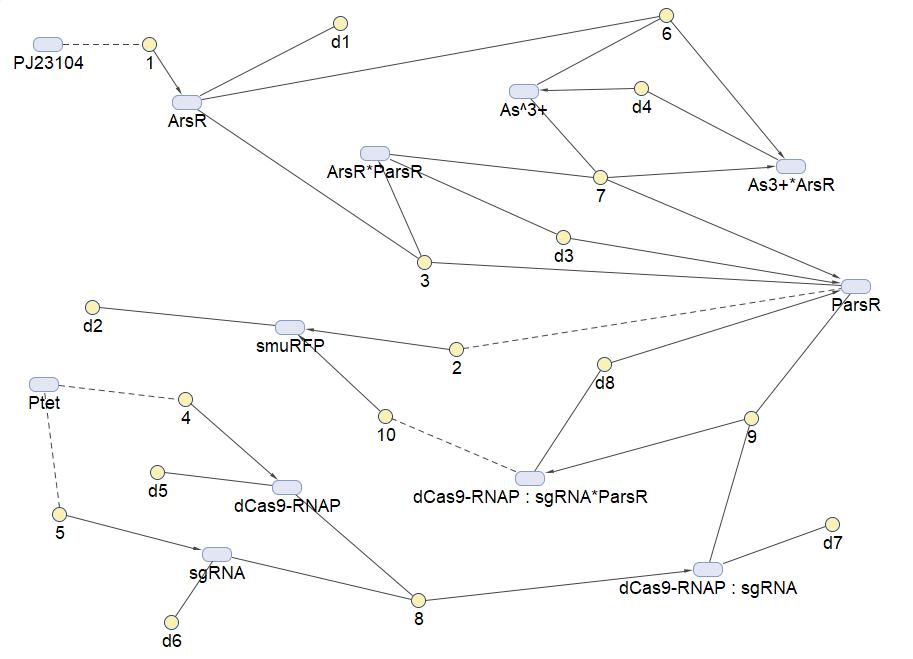
\includegraphics[width=10cm,height=5cm]{screenshot003}	
	\caption{reaction map generated from the reaction set above using SimBiology Toolbox}
\end{figure}

\begin{figure}[h]
	\centering
	\includegraphics[width=10cm,height=5cm]{screenshot002}
	\caption{Schematic diagram of smURFP fluorescence}
\end{figure}




\end{document}


The symbol declaration is:\\\\
$P_{arsR}$: a promoter, which can bind with protein ArsR \\
$GFP_l$: leaking expression without the expression of $As^{3+}$\\
$GFP_r$: reporting expression at the presence of $As^{3+}$\\
\\\\

	k1 & 1.999e-5 &1/s \\
k2 & 3.312e-6 &1/s \\
k3 & 3.3e7    & 1/M    \\
k-3  \\
k4 &1.995e-5 &1/s\\
k5 & 3.312e-6 &1/s \\
k6 &1.66e7   &1/M  \\
k-6 \\
k7  &1.26e4 &1/s  \\
k-7  \\
k8&1.6e-2& 1/s\\
k-8   \\
k9 &1.66e-5&1/s\\ 
k-9\\
k10&4e-5&1/s\\
kd1 & 3.07e-3&1/s\\
kd2&1e-5&1/s\\
kd3&1e-3&1/s\\
kd4&1.53e-3&1/s\\
kd5 & 2e-2&1/s\\
kd6&7.62e-3&1/s\\
kd7& 1e-2&1/s\\
kd8&1e-1&1/s\\

\subsection {advanced edition} 
take the afflux and efflux system into consideration.

\begin{equation}
GlpF\stackrel{k_{11}}{\longrightarrow}GlpF+As^{3+}
\end{equation}

\begin{equation}
ArsB+As^{3+}\stackrel{k_{12}}{\longrightarrow}ArsB
\end{equation}



\subsection{solutions and implication}

\begin{equation}
\frac{d[P_{arsR_u}]}{dt}=-k_1[P_{arsR_u}]\tag{1}
\end{equation}

\begin{equation}
\frac{d[ArsR]}{dt}=k_1[P_{arsR_u}]-k_2[P_{arsR}][ArsR]\tag{2}
\end{equation}

\begin{equation}
\frac{d[GFP_l]}{dt}=k_1[P_{arsR_u}]\tag{3}
\end{equation}

\begin{equation}
\frac{d[ArsR*P_{arsR}]}{dt}=k_2[P_{arsR}][ArsR]-k_4[ArsR*P_{arsR} ][As^{3+}] \tag{4}
\end{equation}

\begin{equation}
\frac{d[plasmid2]}{dt}=-k_3[plasmid2]\tag{5}
\end{equation}

\begin{equation}
\frac{d[RNAP]}{dt}=k_3[plasmid2]-k_5[P_{arsR_d}][RNAP]\tag{6}
\end{equation}

\begin{equation}
\frac{d [RNAP*P_{arsR_d}]}{dt}=k_5[P_{arsR_d}][RNAP]-k_6[RNAP*P_{arsR_d}]\tag{7}
\end{equation}

\begin{equation}
\frac{d [GFP_r]}{dt}=k_6[RNAP*P_{arsR_d}]\tag{8}
\end{equation}